
\documentclass[
dvipsnames, table,   % xcolor option
format=acmsmall,     % paper format
anonymous=true,      % Whether to make author(s) anonymous - used with review below to make anon
authorversion=false, % Whether to generate a special version for the authors’ personal use or posting
]{acmart}

% author-year citation style (required by TELO)
\citestyle{acmauthoryear}

% algorithms
\usepackage{algcompatible, algorithm}
\usepackage[noend]{algpseudocode}
\usepackage{import}
% spacing after full stops in \eg, \ie
\usepackage{xspace}

% subcaptions for side-by-side algorithms
\usepackage[]{subcaption}
\DeclareCaptionSubType*{algorithm}
\renewcommand\thesubalgorithm{\thealgorithm\alph{subalgorithm}}

% table and siunits
\usepackage{tabularx, siunitx}



% best technique and join best labels
%\newcommand{\best}{\color{red}}
%\newcommand{\statsimilar}{\color{blue}}

\begin{document}
\section{Inverted generational distance measurement}
\subsection{WFG1}
\begin{figure}[h]
    \centering
    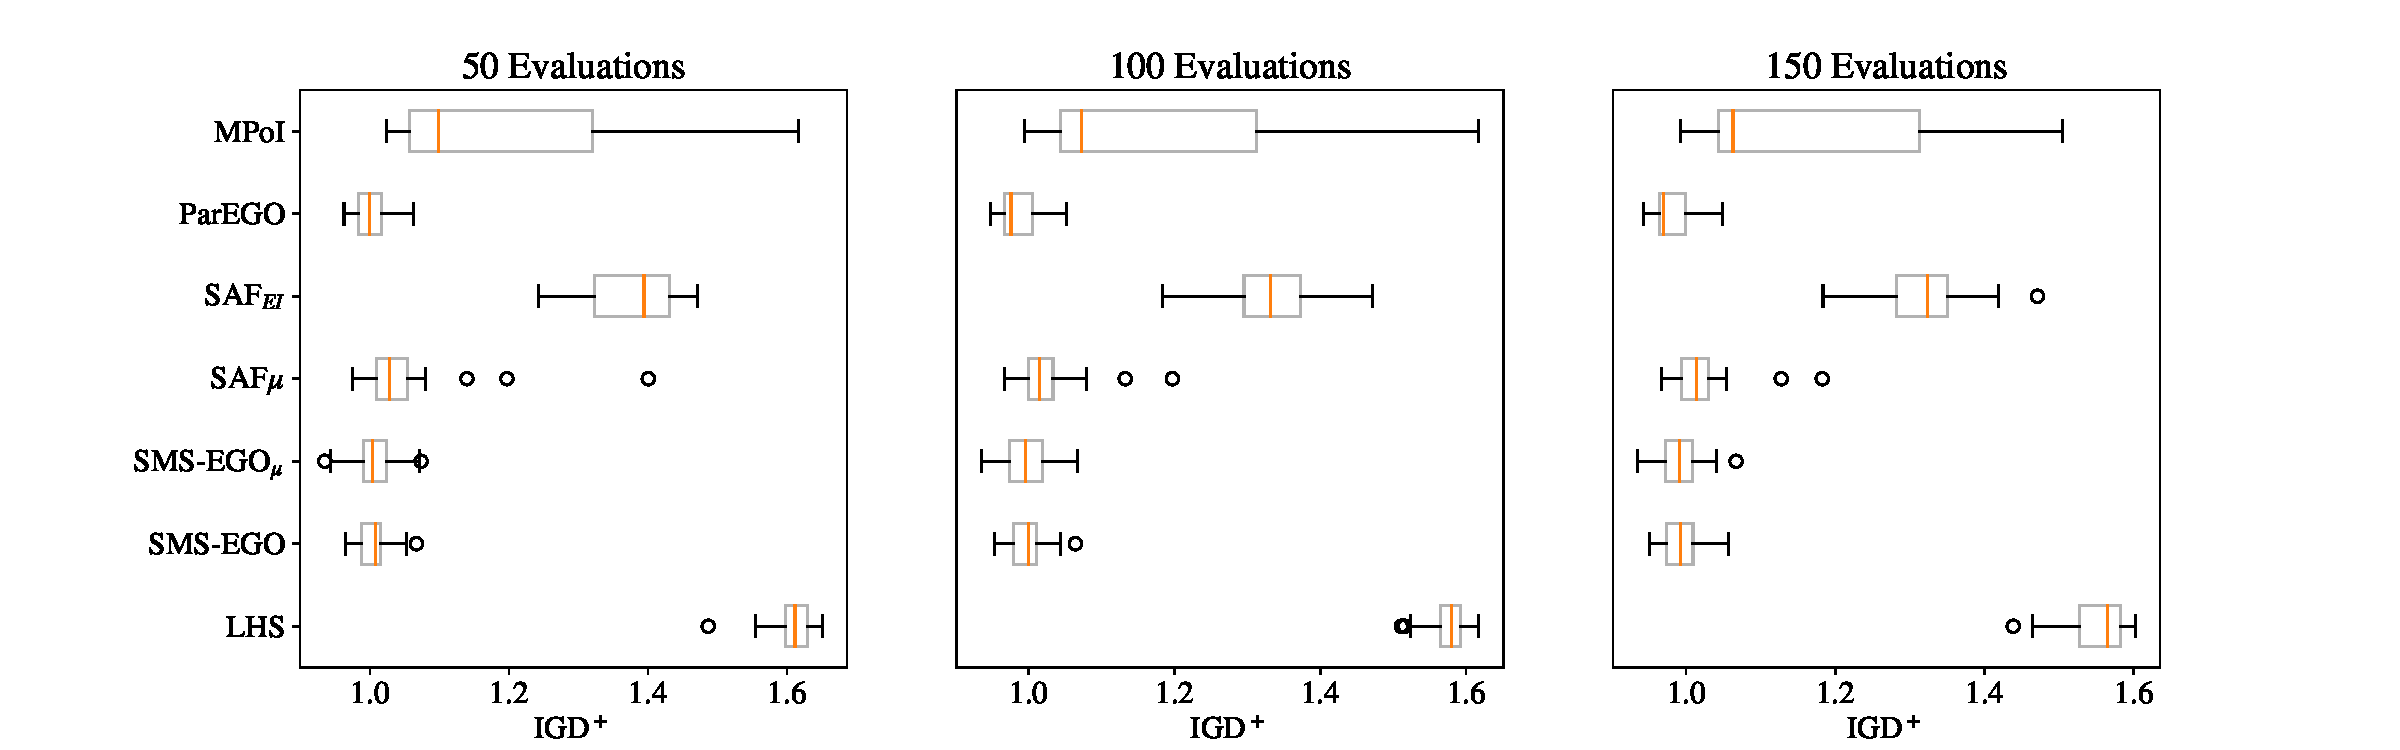
\includegraphics[width=\textwidth]{figures/wfg1_2obj_3dim_igd_boxplot.pdf}
    \caption{WFG1 2obj}
    \label{fig:boxplot WFG1_2obj_3dim}
\end{figure}

\begin{figure}[h]
    \centering
    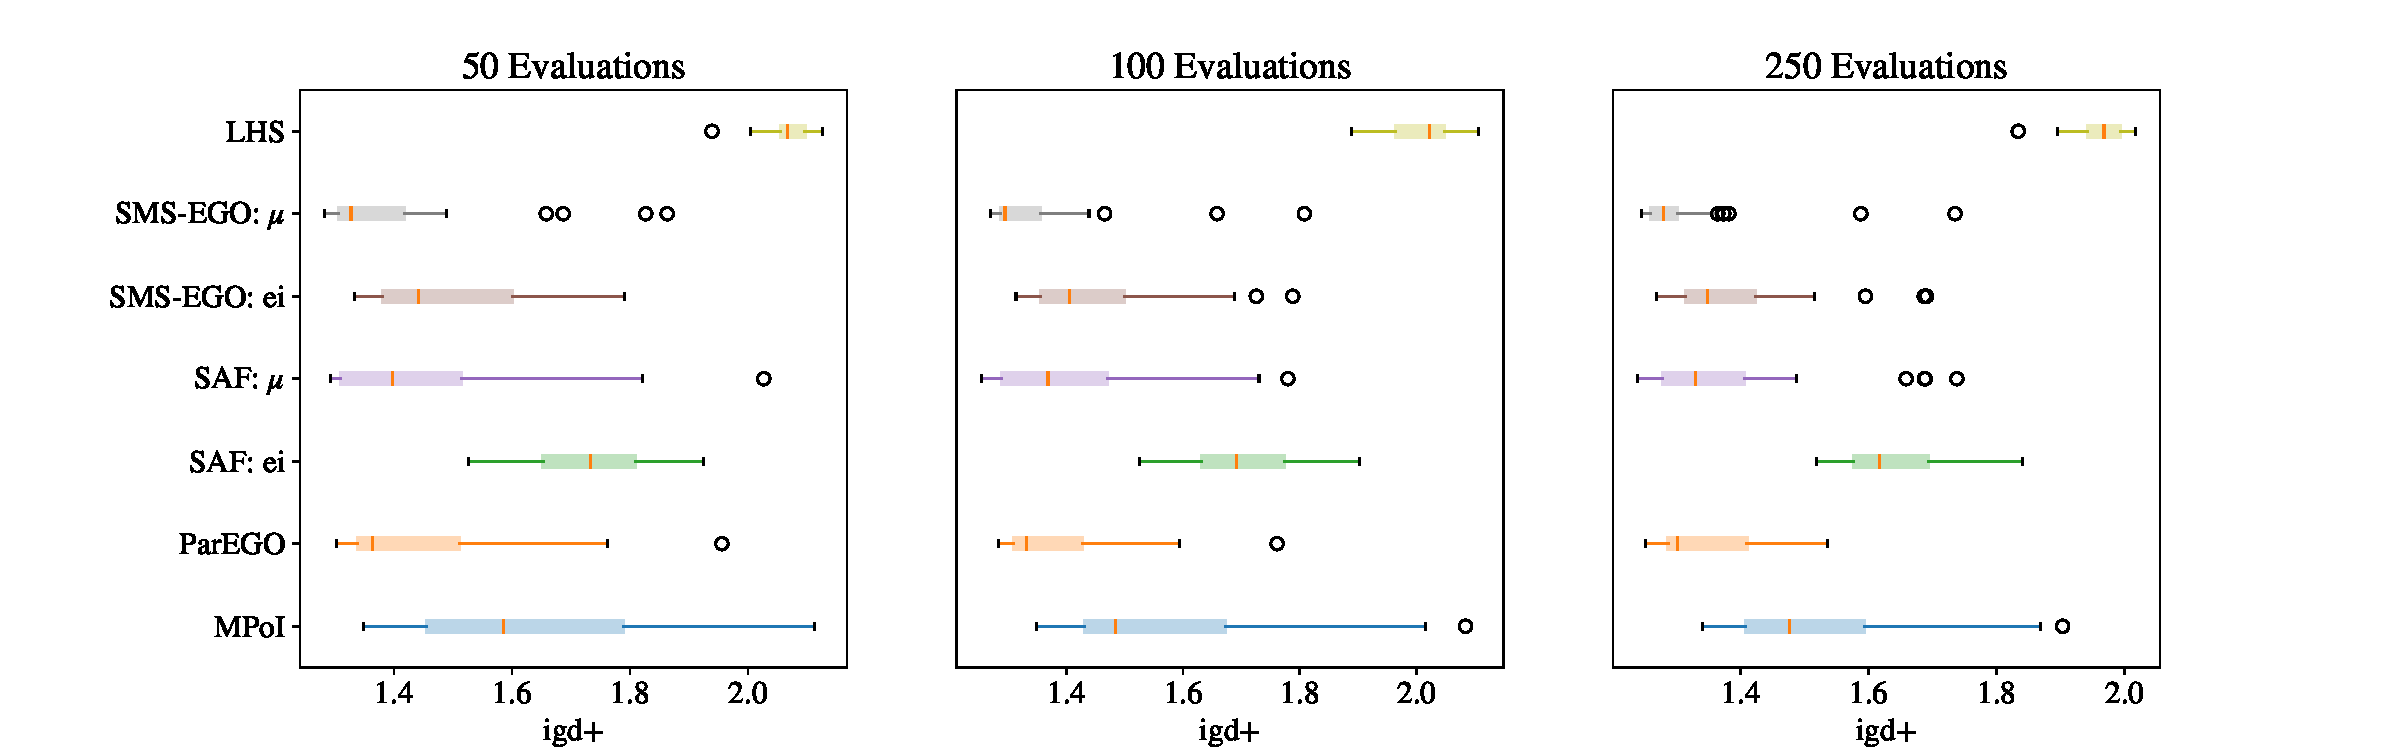
\includegraphics[width=\textwidth]{figures/wfg1_3obj_4dim_igd_boxplot.pdf}
    \caption{WFG1 3obj}
    \label{fig:boxplot WFG1_3obj_4dim}
\end{figure}

\begin{figure}[h]
    \centering
    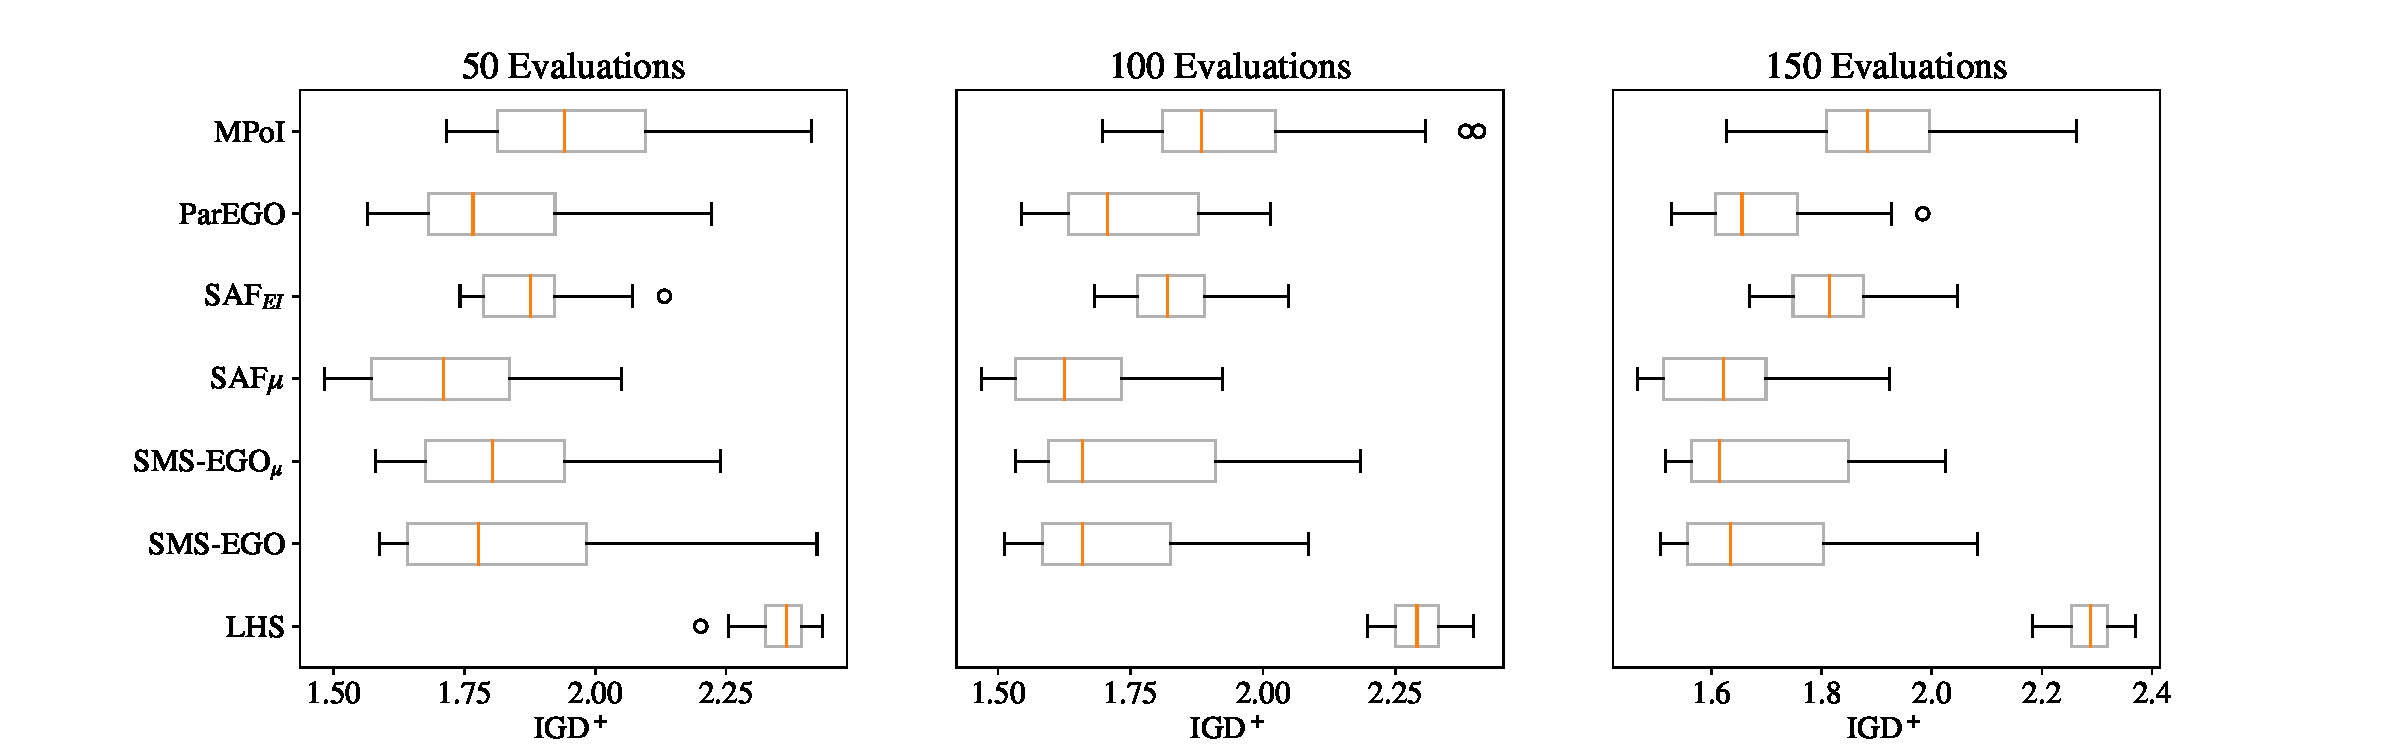
\includegraphics[width=\textwidth]{figures/wfg1_4obj_5dim_igd_boxplot.pdf}
    \caption{WFG1 4obj}
    \label{fig:boxplot WFG1_4obj_5dim}
\end{figure}
\clearpage

\subsection{WFG2}
\begin{figure}[h]
    \centering
    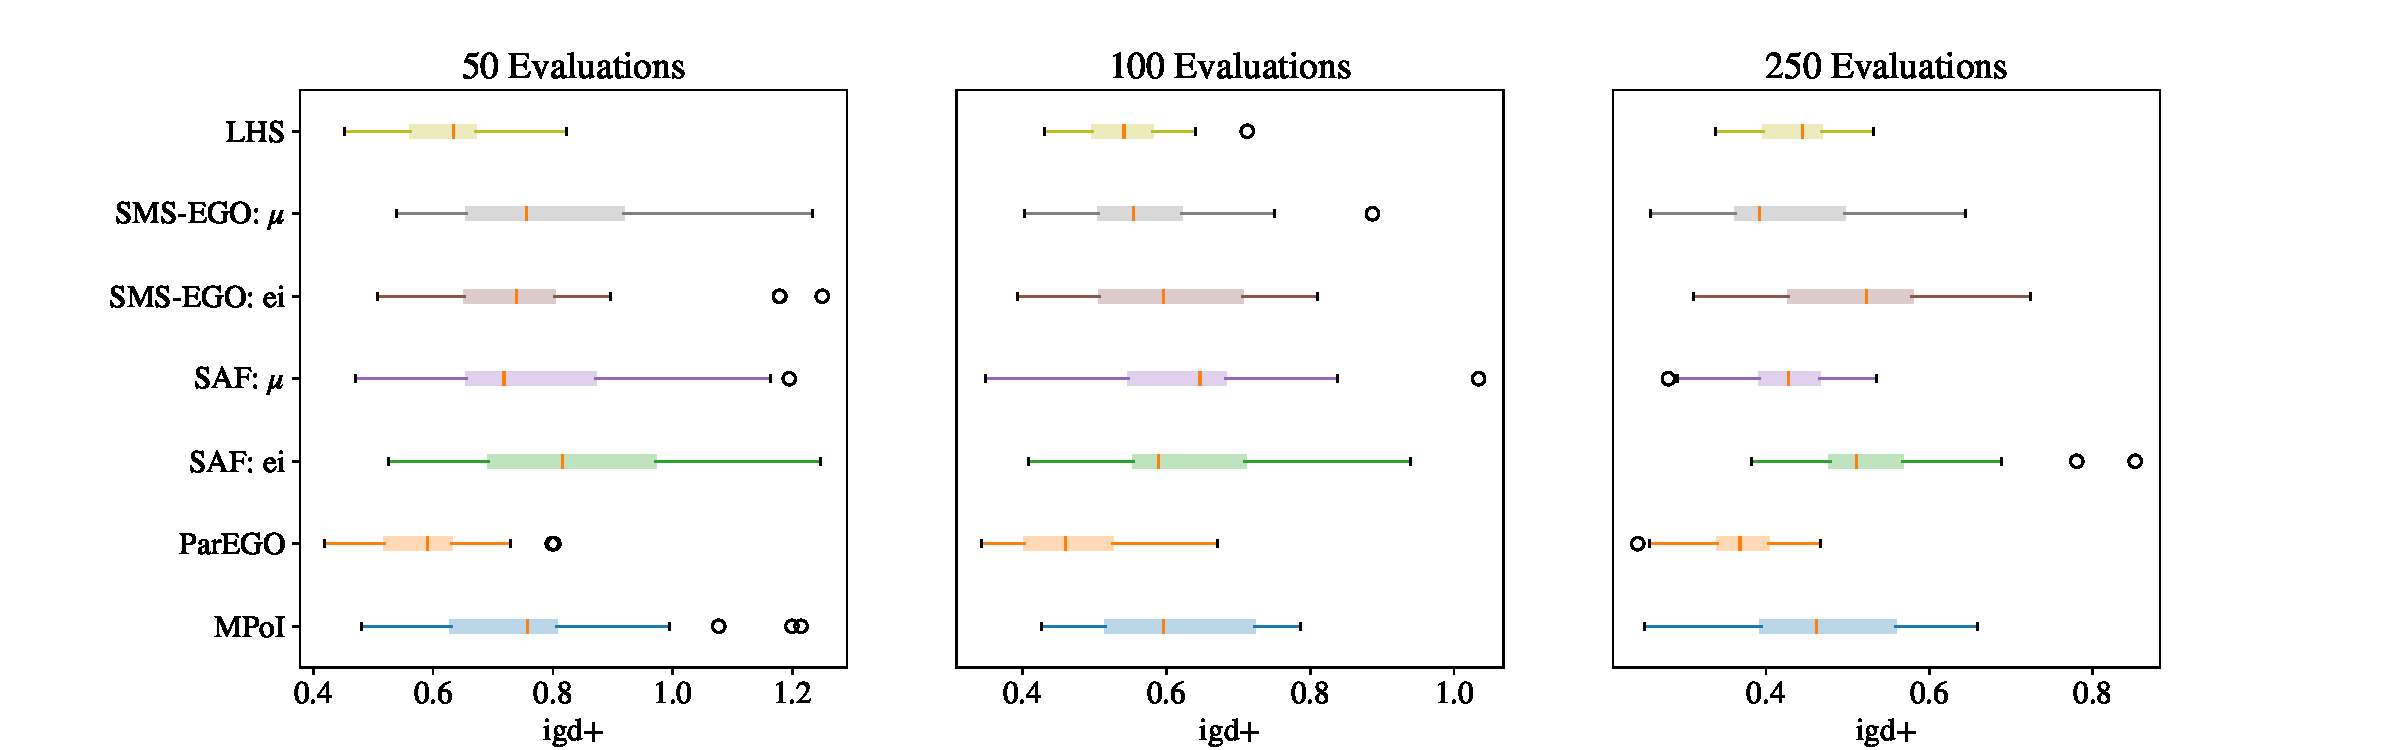
\includegraphics[width=\textwidth]{figures/wfg2_2obj_6dim_igd_boxplot.pdf}
    \caption{WFG2 2obj}
    \label{fig:boxplot WFG2_2obj_6dim}
\end{figure}

\begin{figure}[h]
    \centering
    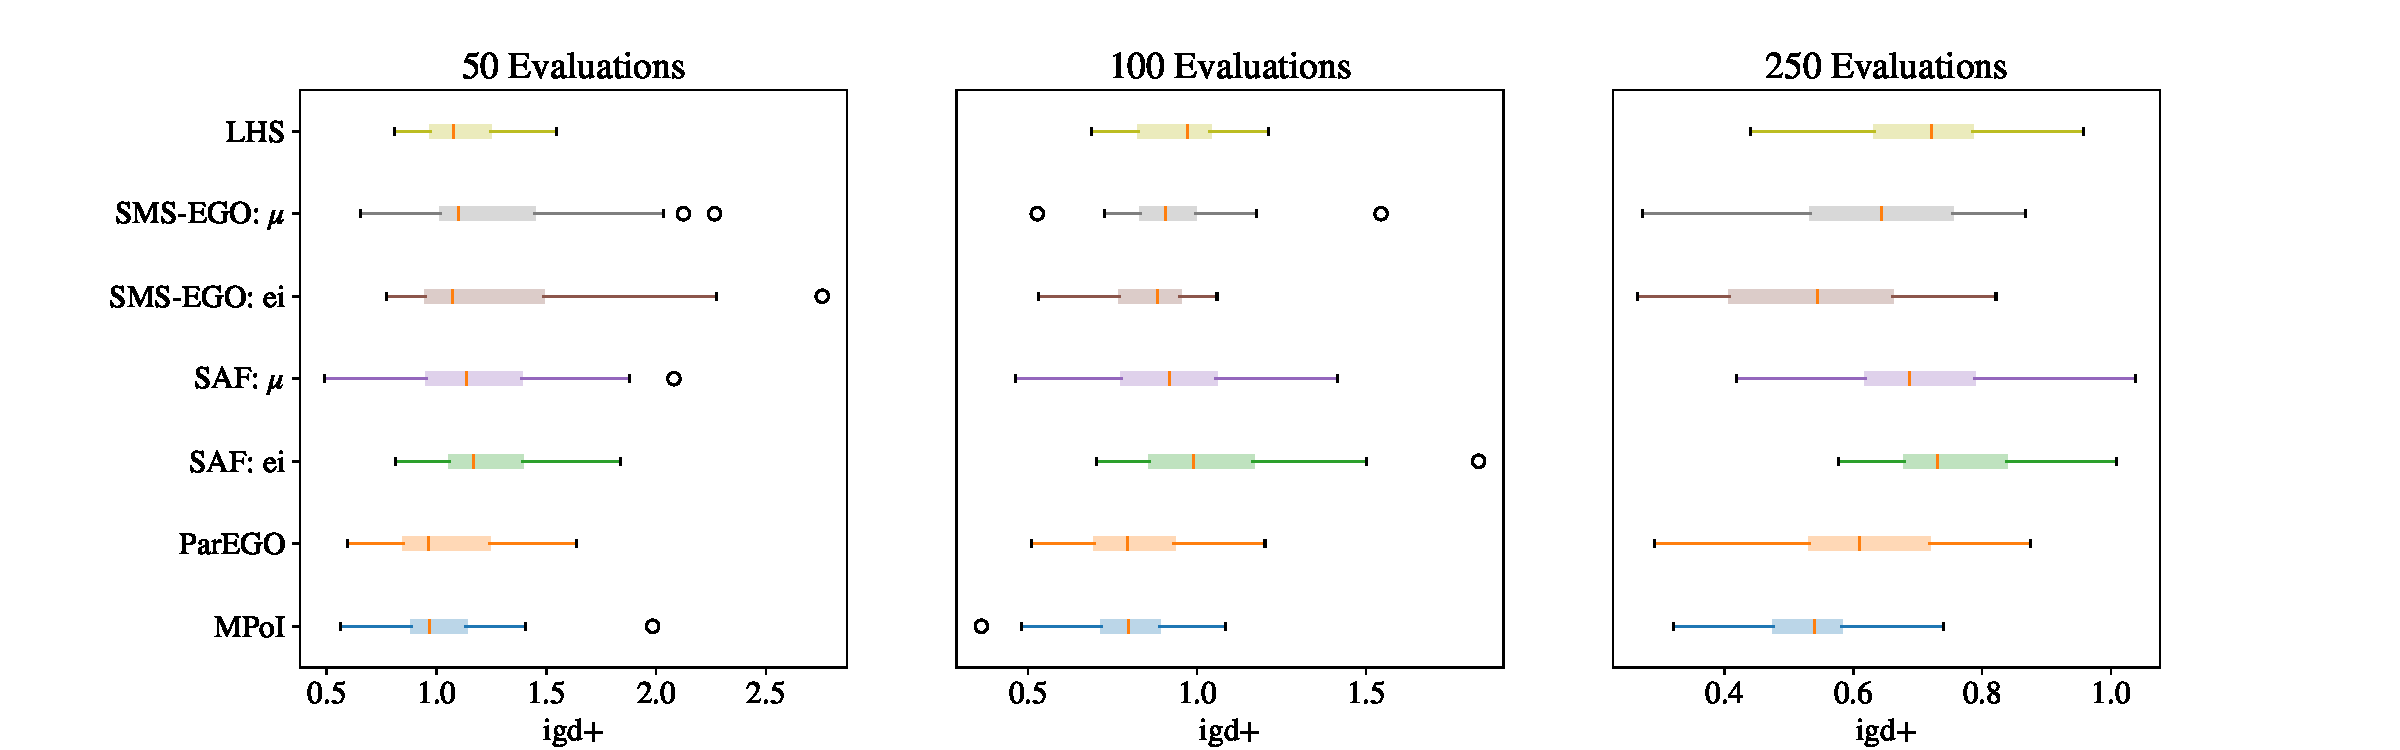
\includegraphics[width=\textwidth]{figures/wfg2_3obj_6dim_igd_boxplot.pdf}
    \caption{WFG2 3obj}
    \label{fig:boxplot WFG2_3obj_6dim}
\end{figure}

\begin{figure}[h]
    \centering
    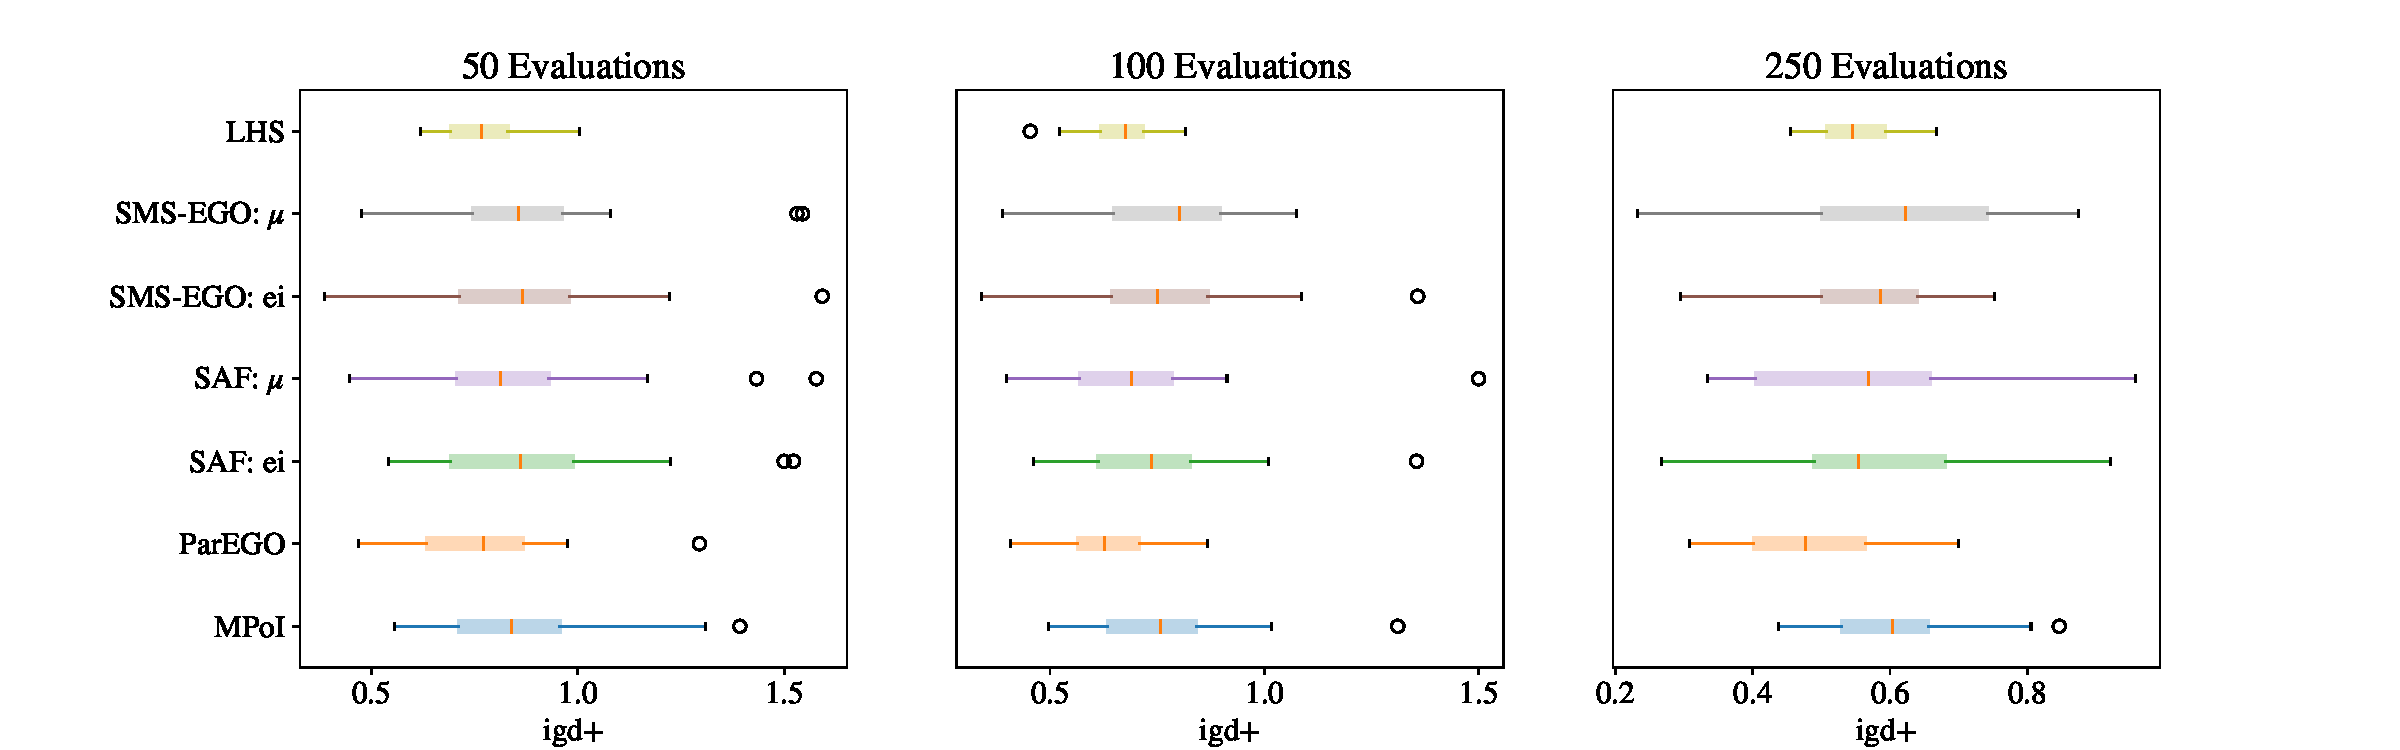
\includegraphics[width=\textwidth]{figures/wfg2_4obj_10dim_igd_boxplot.pdf}
    \caption{WFG2 4obj}
    \label{fig:boxplot WFG2_4obj_10dim}
\end{figure}
\clearpage

\subsection{WFG3}
\begin{figure}[h]
    \centering
    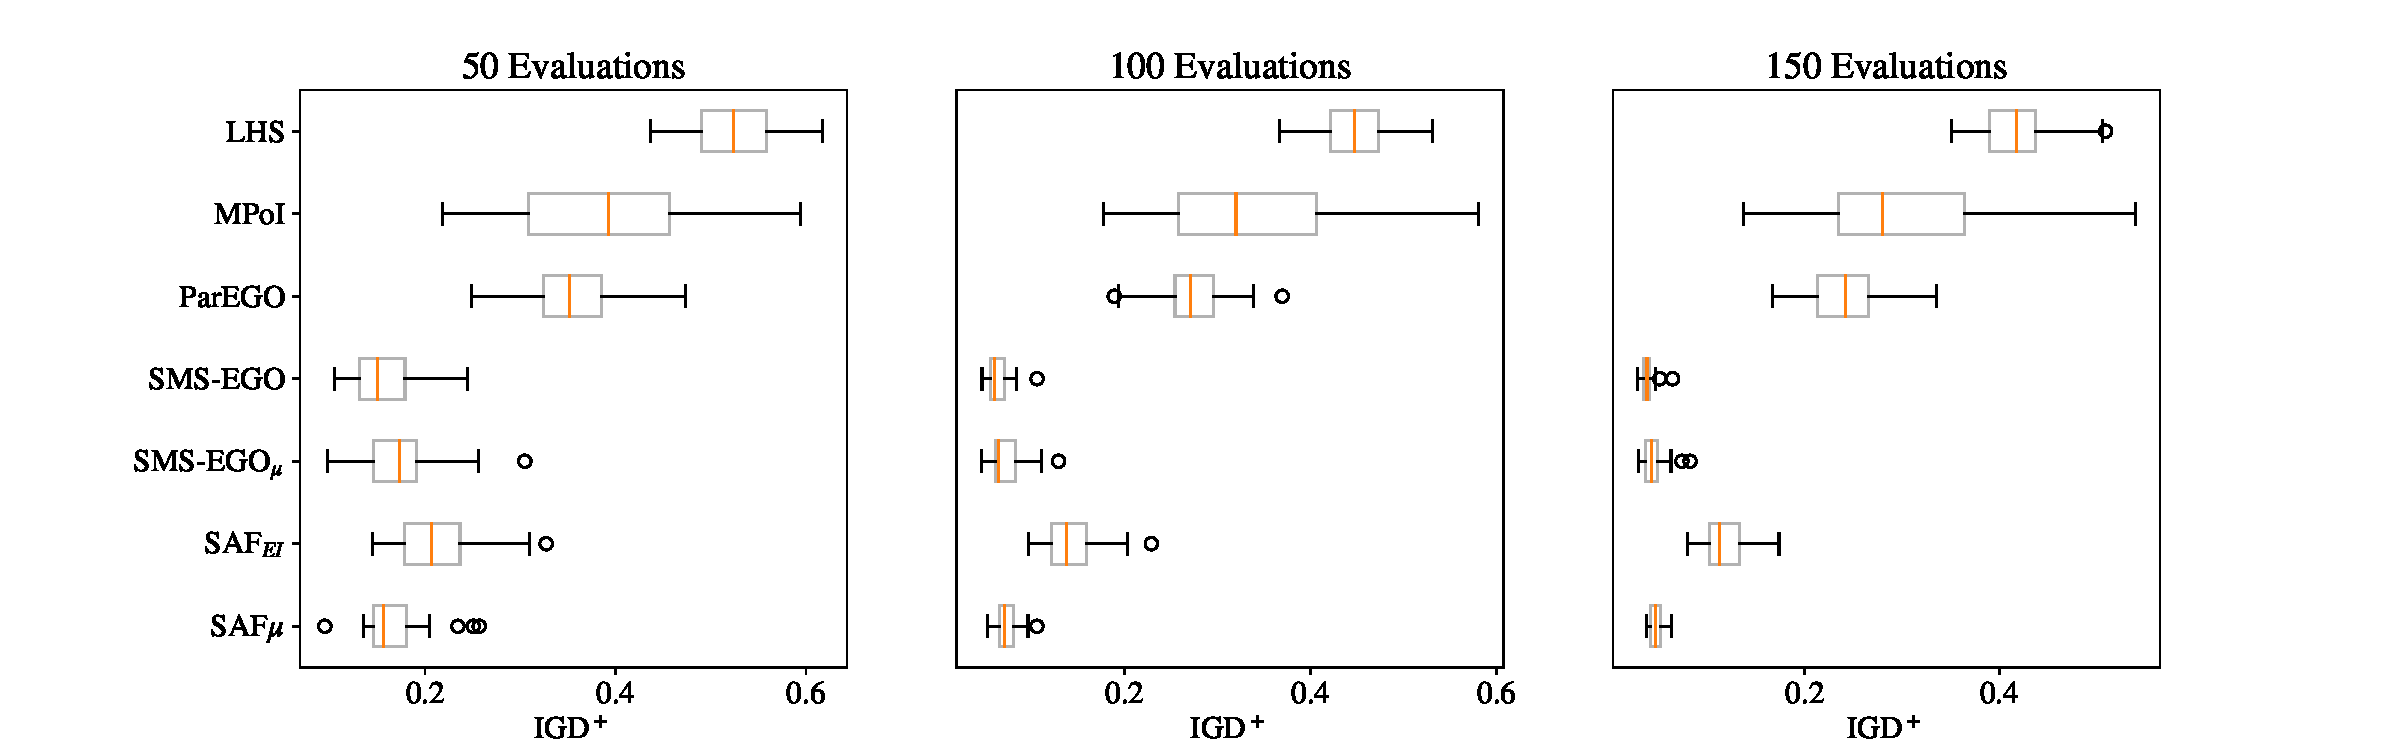
\includegraphics[width=\textwidth]{figures/wfg3_2obj_6dim_igd_boxplot.pdf}
    \caption{WFG3 2obj}
    \label{fig:boxplot WFG3_2obj_6dim}
\end{figure}

\begin{figure}[h]
    \centering
    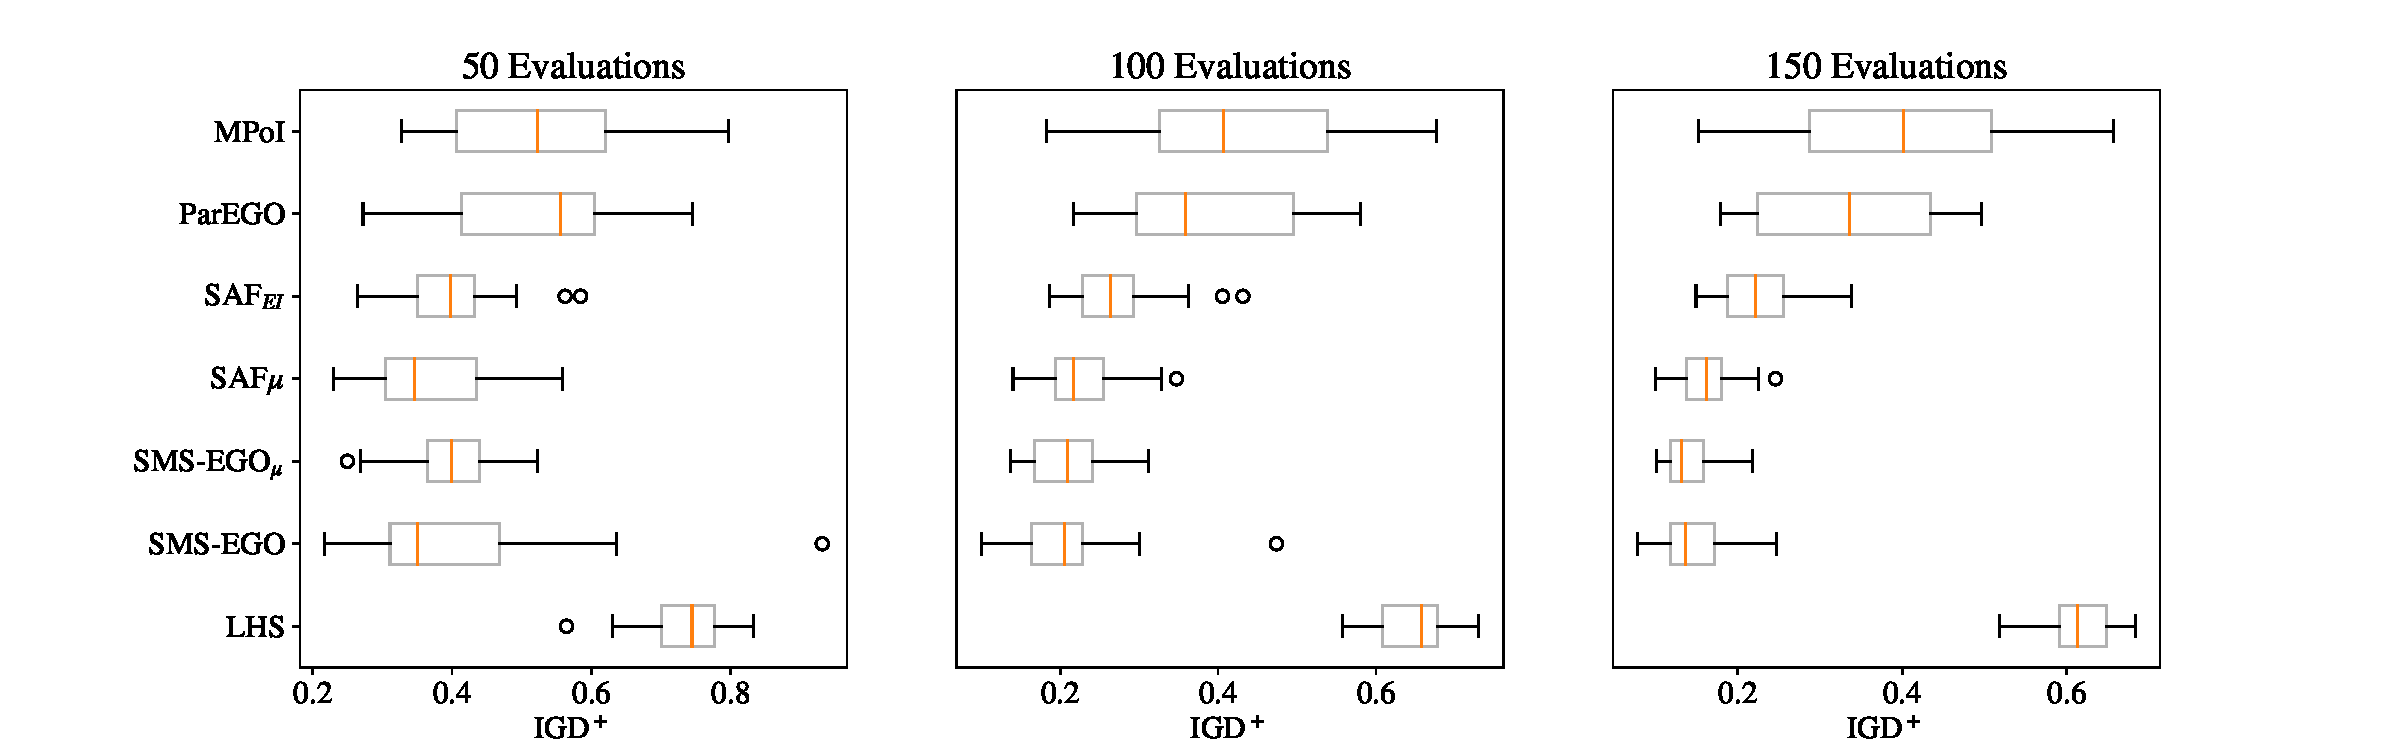
\includegraphics[width=\textwidth]{figures/wfg3_3obj_10dim_igd_boxplot.pdf}
    \caption{WFG3 3obj}
    \label{fig:boxplot WFG3_3obj_10dim}
\end{figure}

\begin{figure}[h]
    \centering
    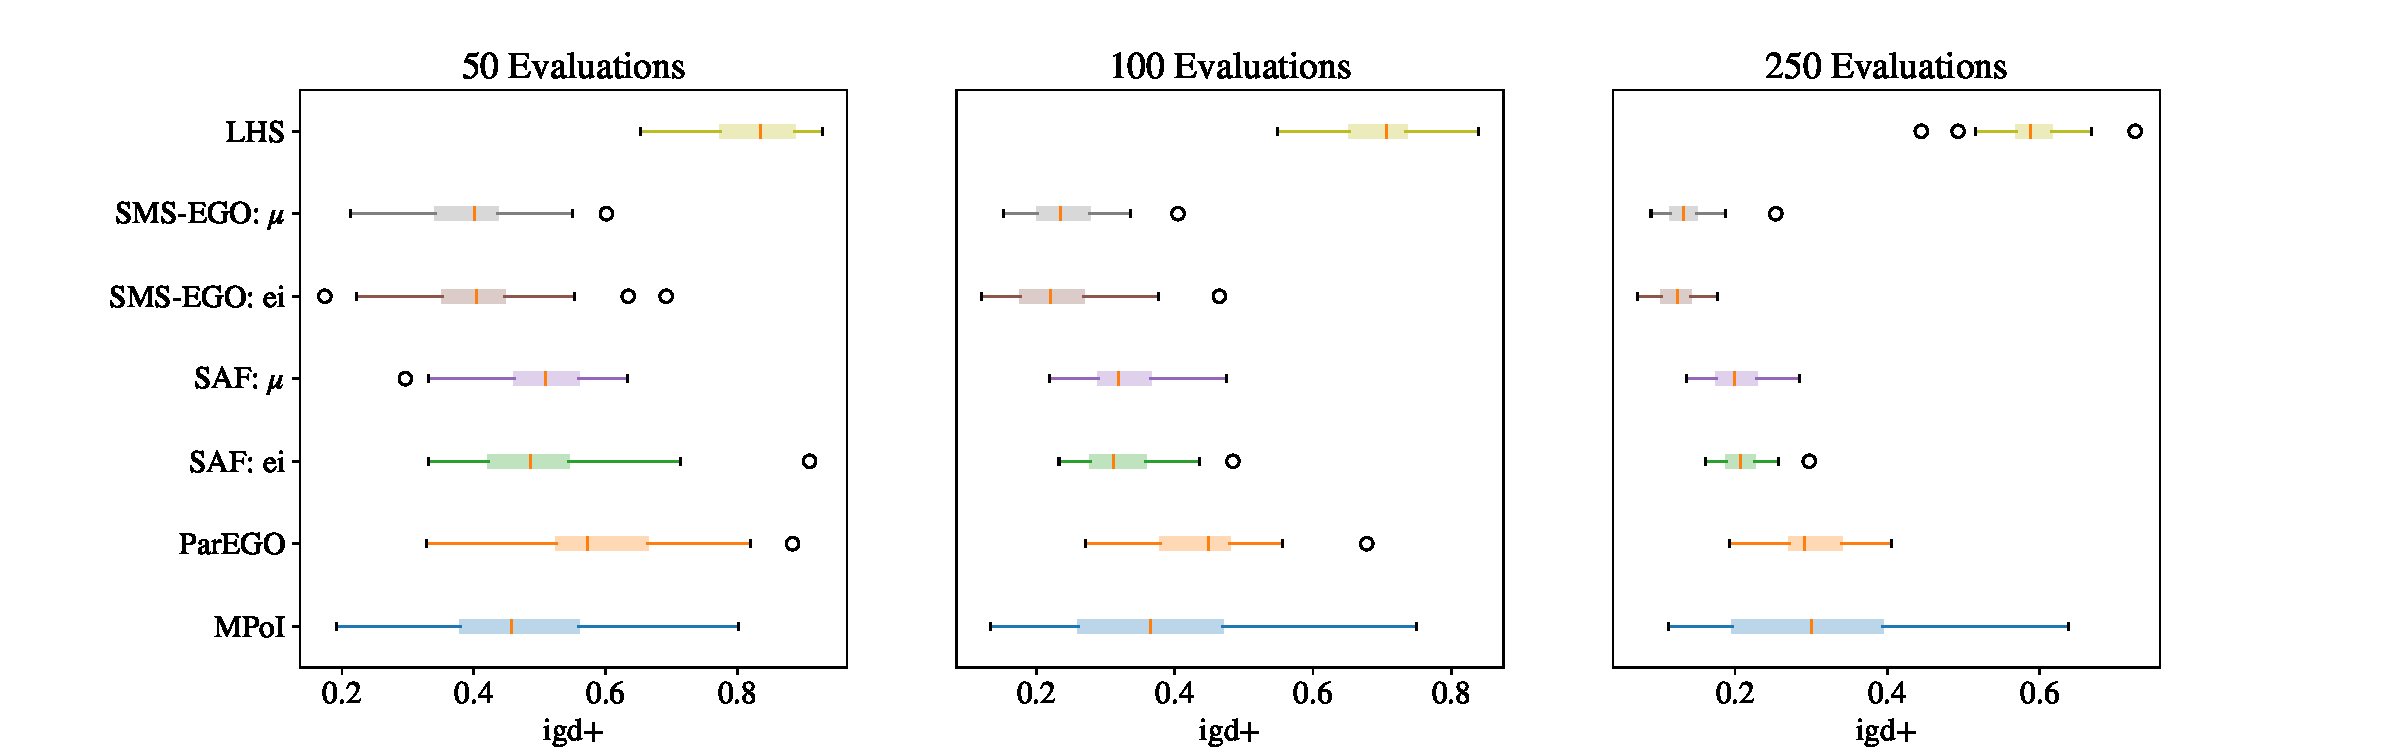
\includegraphics[width=\textwidth]{figures/wfg3_4obj_10dim_2_igd_boxplot.pdf}
    \caption{WFG3 4obj}
    \label{fig:boxplot WFG3_4obj_10dim}
\end{figure}
\clearpage

\subsection{WFG4}
\begin{figure}[h]
    \centering
    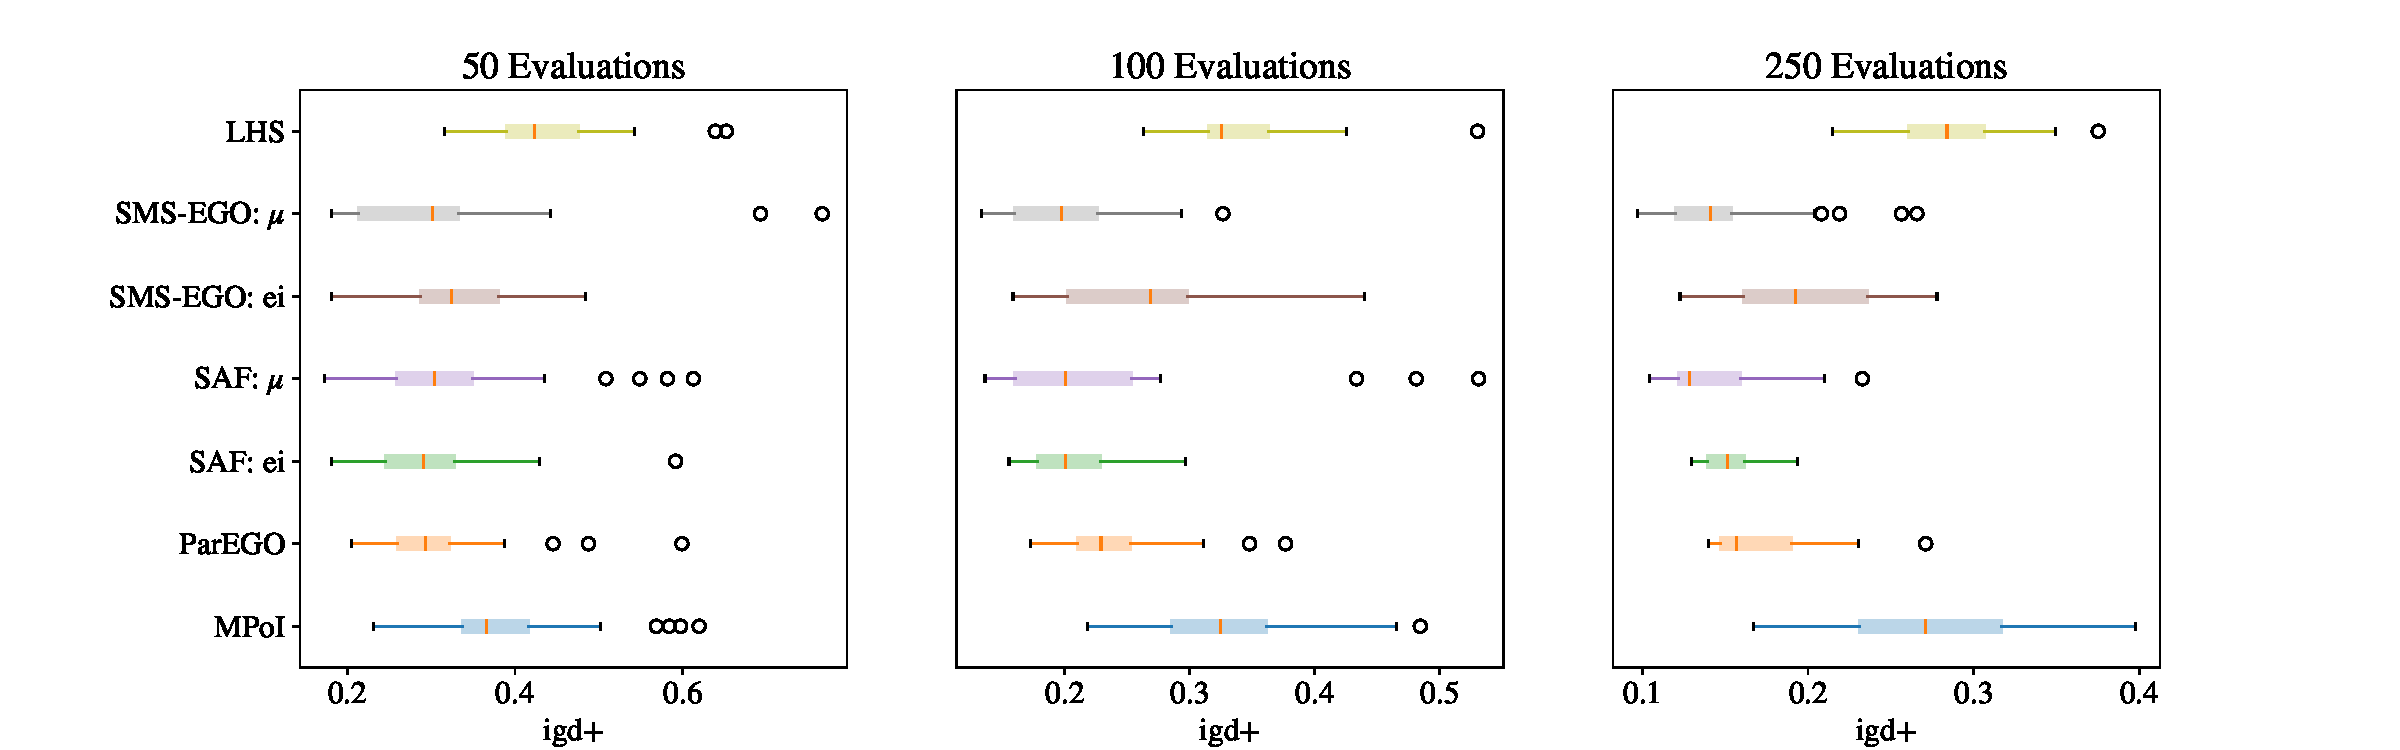
\includegraphics[width=\textwidth]{figures/wfg4_2obj_6dim_igd_boxplot.pdf}
    \caption{WFG4 2obj}
    \label{fig:boxplot WFG4_2obj_6dim}
\end{figure}

\begin{figure}[h]
    \centering
    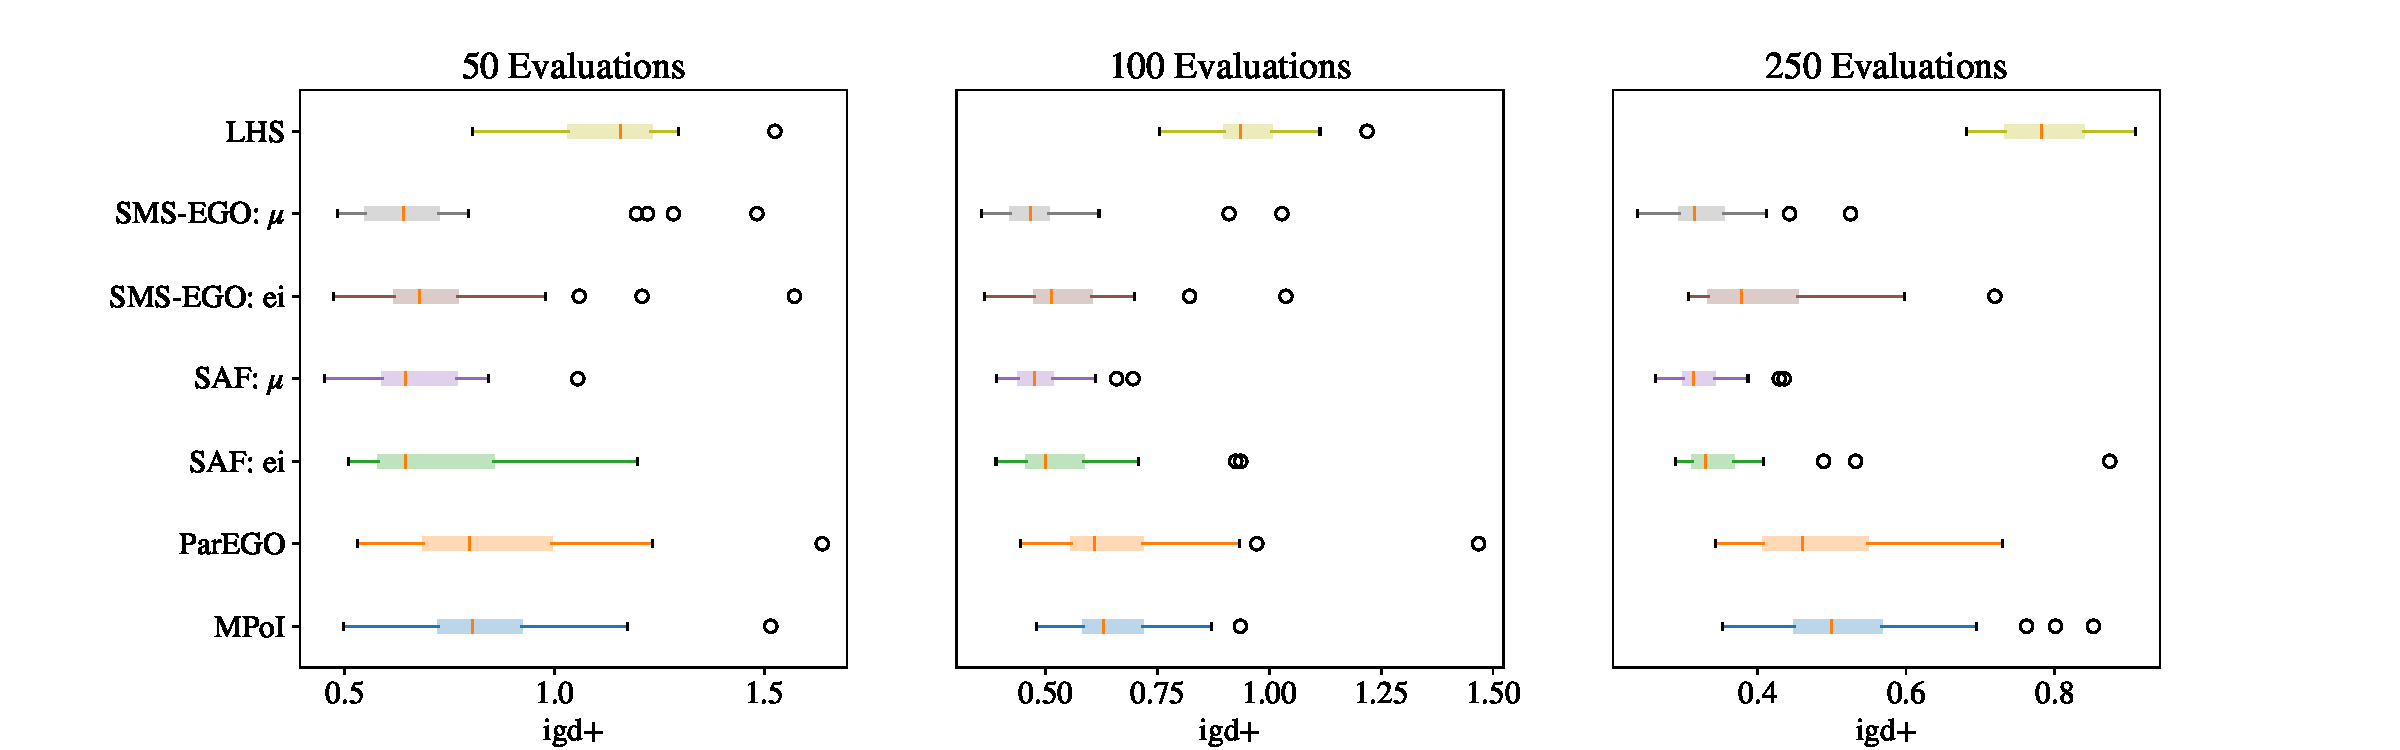
\includegraphics[width=\textwidth]{figures/wfg4_3obj_8dim_igd_boxplot.pdf}
    \caption{WFG4 3obj}
    \label{fig:boxplot WFG4_3obj_8dim}
\end{figure}

\begin{figure}[h]
    \centering
    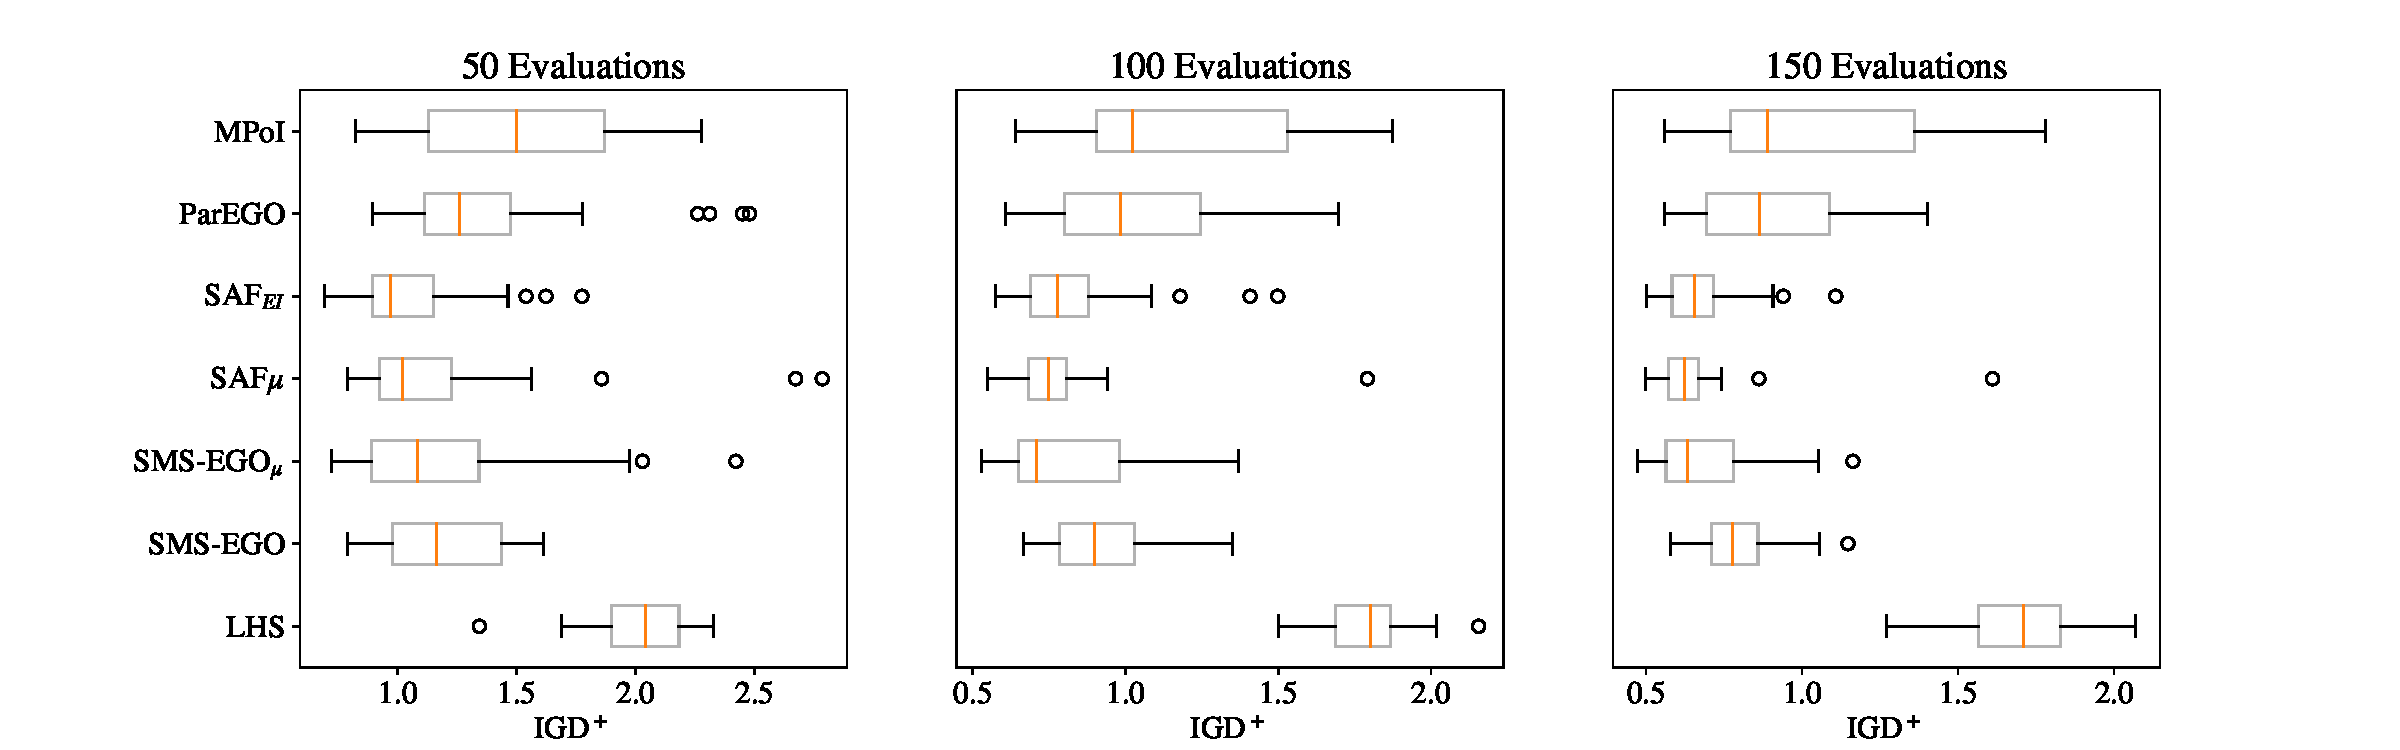
\includegraphics[width=\textwidth]{figures/wfg4_4obj_8dim_igd_boxplot.pdf}
    \caption{WFG4 4obj}
    \label{fig:boxplot WFG4_4obj_8dim}
\end{figure}



\end{document}
%%% Local Variables:
%%% mode: latex
%%% TeX-master: t
%%% auto-fill-mode: t
%%% End: